\documentclass[a4paper,11pt]{article}

\usepackage{amsmath}
\usepackage{graphicx}
\usepackage{listings}
\usepackage{xcolor}
\usepackage{booktabs}
\usepackage{multirow}
\usepackage{caption}
\usepackage{cite}     % For numeric citations
\usepackage{url}      % Needed for proper URL handling
\usepackage{pgfplots} % For creating plots
\usepackage{tikz}     % Required for pgfplots
\usepackage{hyperref}  % Load hyperref last (it includes url functionality)

\pgfplotsset{compat=1.16} % Set compatibility mode for pgfplots

\hypersetup{
    colorlinks=true,
    linkcolor=blue,
    filecolor=magenta,      
    urlcolor=cyan,
    citecolor=blue,        % Set citation numbers to blue color
    pdftitle={PID Control and Auto-Tuning in the VentCon Pressure Control System},
    pdfauthor={VENTREX},
}

\definecolor{codegreen}{rgb}{0,0.6,0}
\definecolor{codegray}{rgb}{0.5,0.5,0.5}
\definecolor{codepurple}{rgb}{0.58,0,0.82}
\definecolor{backcolour}{rgb}{0.95,0.95,0.95}

\lstdefinestyle{mystyle}{
    backgroundcolor=\color{backcolour},   
    commentstyle=\color{codegreen},
    keywordstyle=\color{magenta},
    numberstyle=\tiny\color{codegray},
    stringstyle=\color{codepurple},
    basicstyle=\ttfamily\footnotesize,
    breakatwhitespace=false,         
    breaklines=true,                 
    captionpos=b,                    
    keepspaces=true,                 
    numbers=left,                    
    numbersep=5pt,                  
    showspaces=false,                
    showstringspaces=false,
    showtabs=false,                  
    tabsize=2
}

\lstset{style=mystyle}

\title{PID Control and Auto-Tuning in the VentCon Pressure Control System}
\author{VENTREX}
\date{\today}

\begin{document}

\maketitle

\begin{abstract}
This document describes the implementation of the PID (Proportional-Integral-Derivative) control system and auto-tuning procedures in the VentCon pressure control system. The document details the core control algorithm, anti-windup mechanisms, hysteresis compensation, and the relay-based auto-tuning method with multiple tuning rules for different performance requirements.
\end{abstract}

\tableofcontents

\section{Introduction}

The VentCon2 system is designed to provide precise pressure control using a solenoid valve operated via PWM (Pulse Width Modulation). The system employs a digital PID controller to maintain the desired pressure setpoint by dynamically adjusting the valve opening based on real-time pressure measurements. To simplify the tuning process, an automated self-tuning procedure based on the relay method is implemented.

\section{PID Control Implementation}

\subsection{Basic PID Theory}

The PID control algorithm calculates the control output $u(t)$ based on the error $e(t)$ between the desired setpoint and the measured process variable\cite{wiki:pid}:

\begin{equation}
u(t) = K_p e(t) + K_i \int_{0}^{t} e(\tau) d\tau + K_d \frac{de(t)}{dt}
\end{equation}

Where:
\begin{itemize}
    \item $K_p$ is the proportional gain
    \item $K_i$ is the integral gain
    \item $K_d$ is the derivative gain
    \item $e(t) = \text{setpoint} - \text{measured value}$
\end{itemize}

\subsection{Implementation in VentCon2}

The VentCon2 system uses the PID\_v2 library for Arduino which implements a discrete form of the PID equation. The controller is configured with the following parameters:

\begin{lstlisting}[language=C++, caption=PID Configuration]
// PID initialization
PID pid(&pressureInput, &pwmOutput, &settings.setpoint, 
        settings.Kp, settings.Ki, settings.Kd, DIRECT);
pid.SetMode(PID::Automatic);
pid.SetOutputLimits(0, pwm_max_value);
pid.SetSampleTime(SAMPLE_TIME); // 10ms (100Hz)
\end{lstlisting}

The controller updates at a frequency of 100Hz, providing excellent responsiveness while maintaining processing efficiency. The PID output is then mapped to the valve's effective operating range (50\% to 90\% duty cycle), as the valve exhibits non-linear behavior at lower duty cycles.

\subsection{Anti-Windup Implementation}

The system implements an advanced anti-windup mechanism that prevents integral windup in two key situations:

\begin{enumerate}
    \item When the valve is below its minimum effective operating range (50\% duty cycle)
    \item When the valve is above its maximum effective operating range (90\% duty cycle)
\end{enumerate}

The anti-windup mechanism works by temporarily switching the PID controller to manual mode and back to automatic when these conditions are detected, effectively resetting the integral component:

\begin{lstlisting}[language=C++, caption=Anti-Windup Implementation]
if (settings.antiWindup) 
{
  float pidPercent = (pwmOutput / pwm_max_value) * 100.0;
  
  if ((pidPercent < VALVE_MIN_DUTY && pwmOutput > previousOutput) ||
      (pidPercent > VALVE_MAX_DUTY && pwmOutput > previousOutput)) 
  {
    // Reset the PID to prevent integral accumulation
    pid.SetMode(PID::Manual);
    pid.SetMode(PID::Automatic);
  }
}
\end{lstlisting}

\subsection{Hysteresis Compensation}

Solenoid valves typically exhibit hysteresis behavior, where the opening and closing characteristics differ. To compensate for this, the system implements a direction-based hysteresis compensation mechanism:

\begin{lstlisting}[language=C++, caption=Hysteresis Compensation]
if (settings.hysteresis) 
{
  bool currentlyIncreasing = pressureInput > lastPressure;
  
  if (currentlyIncreasing != pressureIncreasing) 
  {
    if (!currentlyIncreasing) 
    {
      // When changing direction from increasing to decreasing
      pidPercent += settings.hystAmount;
    }
    else 
    {
      // When changing direction from decreasing to increasing
      pidPercent -= settings.hystAmount;
    }
    
    pressureIncreasing = currentlyIncreasing;
  }
}
\end{lstlisting}

This approach helps overcome the "stiction" effect in solenoid valves, providing more consistent control regardless of whether the pressure is increasing or decreasing.

\section{Auto-Tuning Procedure}

\subsection{Relay Method Theory}

The auto-tuning implementation uses the relay method developed by Åström and Hägglund\cite{astrom1984automatic}, which is a variation of the Ziegler-Nichols frequency response method\cite{ziegler1942optimum}. This approach is widely used in industrial applications due to its reliability and ease of implementation\cite{wiki:pidtuning}. Instead of increasing the proportional gain until sustained oscillation occurs (which can be difficult and potentially unsafe), the relay method:

\begin{enumerate}
    \item Forces the system into controlled oscillation using a relay (on/off) controller
    \item Measures the resulting oscillation amplitude and period
    \item Calculates the "ultimate gain" ($K_u$) and "ultimate period" ($T_u$)
    \item Applies tuning rules to determine the optimal PID parameters
\end{enumerate}

The ultimate gain is calculated as:

\begin{equation}
K_u = \frac{4d}{\pi a}
\end{equation}

Where:
\begin{itemize}
    \item $d$ is the relay amplitude (AUTOTUNE\_RELAY\_HIGH = 90\%)
    \item $a$ is the resulting oscillation amplitude in the process variable
\end{itemize}

\subsection{Relay Method Visualization}

Figure \ref{fig:relay_method} illustrates the relay method auto-tuning process, showing how the relay output forces controlled oscillation in the pressure system and how the key parameters are measured.

\begin{figure}[ht]
\centering
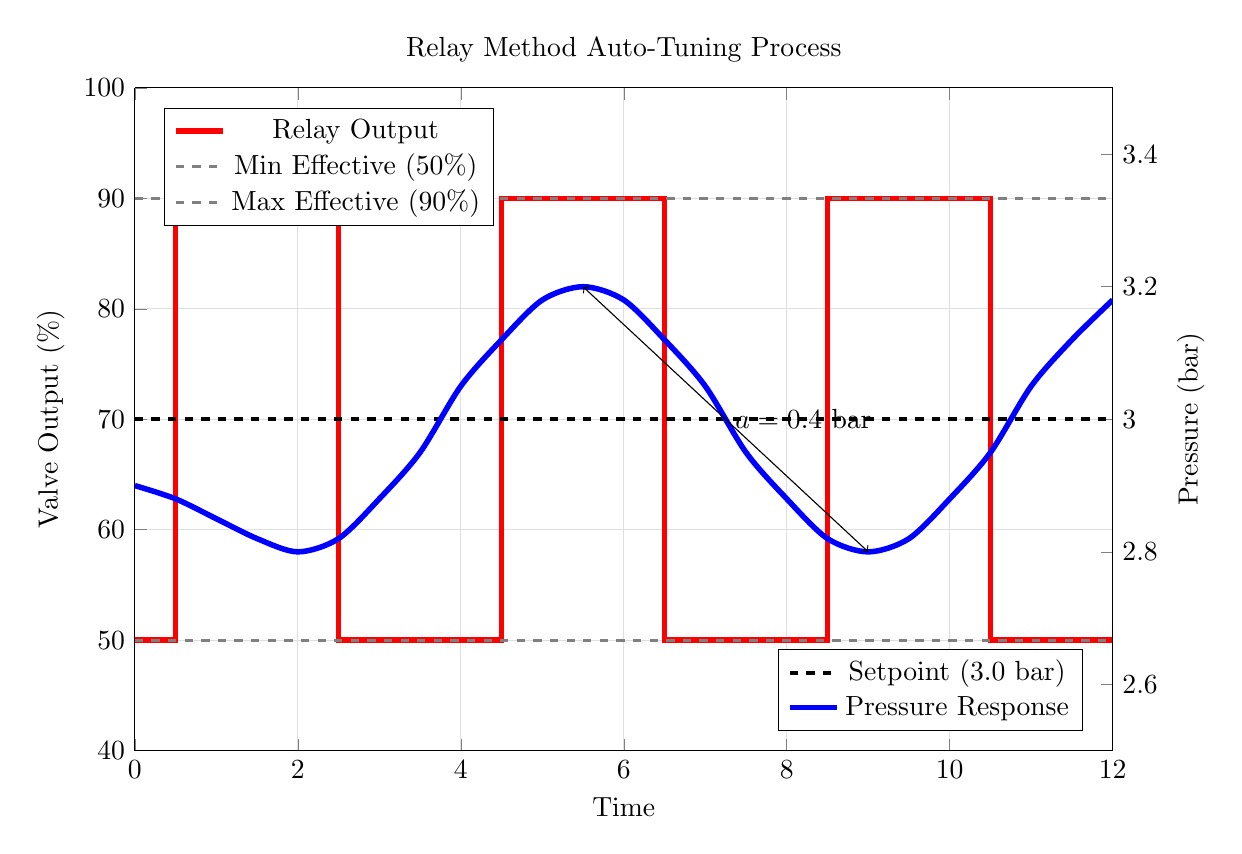
\begin{tikzpicture}
\begin{axis}[
    width=14cm,
    height=10cm,
    xlabel={Time},
    ylabel={Valve Output (\%)},
    xmin=0, xmax=12,
    ymin=40, ymax=100,
    xtick={0,2,4,6,8,10,12},
    ytick={40,50,60,70,80,90,100},
    legend pos=north west,
    grid=both,
    minor grid style={gray!25},
    major grid style={gray!25},
    title={Relay Method Auto-Tuning Process},
    axis y line*=left,
    ]
    
    % Relay output (square wave between 50% and 90%)
    \addplot[red, line width=2pt, mark=none] coordinates {
        (0,50) (0.5,50) (0.5,90) (2.5,90) (2.5,50) (4.5,50) (4.5,90) 
        (6.5,90) (6.5,50) (8.5,50) (8.5,90) (10.5,90) (10.5,50) (12,50)
    };
    
    % Valve effective range markers
    \addplot[gray, dashed, line width=1pt] coordinates {(0,50) (12,50)};
    \addplot[gray, dashed, line width=1pt] coordinates {(0,90) (12,90)};
    
    \legend{Relay Output, Min Effective (50\%), Max Effective (90\%)}
\end{axis}

% Second y-axis for pressure
\begin{axis} [
    width=14cm,
    height=10cm,
    xlabel={},
    ylabel={Pressure (bar)},
    xmin=0, xmax=12,
    ymin=2.5, ymax=3.5,
    xtick=\empty,
    ytick={2.6,2.8,3.0,3.2,3.4},
    legend pos=south east,
    grid=none,
    axis y line*=right,
    axis x line=none,
    ]
    
    % Setpoint line
    \addplot[black, dashed, line width=1.5pt] coordinates {(0,3.0) (12,3.0)};
    
    % Pressure response (sinusoidal-like with phase lag)
    \addplot[blue, line width=2pt, smooth] coordinates {
        (0,2.9) (0.5,2.88) (1,2.85) (1.5,2.82) (2,2.8) (2.5,2.82) 
        (3,2.88) (3.5,2.95) (4,3.05) (4.5,3.12) (5,3.18) (5.5,3.2) 
        (6,3.18) (6.5,3.12) (7,3.05) (7.5,2.95) (8,2.88) (8.5,2.82) 
        (9,2.8) (9.5,2.82) (10,2.88) (10.5,2.95) (11,3.05) (11.5,3.12) (12,3.18)
    };
    
    % Amplitude markers
    \draw[<->] (axis cs:5.5,3.2) -- (axis cs:9,2.8) node[midway,right] {$a = 0.4$ bar};
    
    % Period marker
    \draw[<->] (axis cs:2.5,2.4) -- (axis cs:6.5,2.4) node[midway,below] {$T_u = 4.0$ s};
    
    \legend{Setpoint (3.0 bar), Pressure Response}
\end{axis}
\end{tikzpicture}
\caption{Relay method auto-tuning illustration showing the square wave relay output (red) switching between the valve's effective operating range of 50-90\% and the resulting sinusoidal pressure response (blue). The ultimate period $T_u$ and oscillation amplitude $a$ are measured to calculate the PID parameters.}
\label{fig:relay_method}
\end{figure}

Key observations from the relay method:

\begin{itemize}
    \item \textbf{Relay Output}: Switches between 50\% (minimum effective opening) and 90\% (maximum effective opening) based on pressure relative to setpoint
    \item \textbf{Pressure Response}: Shows sinusoidal oscillation around the setpoint with phase lag relative to the valve output
    \item \textbf{Ultimate Period ($T_u$)}: Measured as the time between consecutive transitions (e.g., 4.0 seconds in the example)
    \item \textbf{Oscillation Amplitude ($a$)}: Peak-to-peak pressure variation (e.g., 0.4 bar in the example)
    \item \textbf{Phase Relationship}: The pressure response lags behind the valve output due to system dynamics
\end{itemize}

The ultimate gain is then calculated as: $K_u = \frac{4 \times (90\% - 50\%)}{\pi \times 0.4 \text{ bar}} = \frac{4 \times 40\%}{\pi \times 0.4} = \frac{160}{1.257} = 127.3$

\subsection{Implementation in VentCon2}

The auto-tuning process in VentCon2 works as follows:

\begin{enumerate}
    \item The system sets the target pressure to a predefined setpoint (3.0 bar)
    \item A relay controller alternates the valve between:
    \begin{itemize}
        \item 50\% (minimum effective opening) when pressure exceeds the setpoint
        \item 90\% of effective valve opening when pressure falls below setpoint - noise band
    \end{itemize}
    \item The system records the cycle times and amplitudes for a configurable number of cycles (default 10) or until timeout
    \item The ultimate gain and period are calculated from the averaged measurements
    \item PID parameters are calculated using the selected tuning rule
\end{enumerate}

An important implementation detail is the handling of the valve's non-linear behavior. The relay amplitude (90\%) refers to the actual valve opening percentage rather than the raw PWM value. When applying the relay output in the high state, the system accounts for the valve's characteristics by mapping this percentage to the appropriate PWM value:

\begin{lstlisting}[language=C++, caption=Auto-Tuning Relay Output]
// When in high state:
float mappedDuty = VALVE_MIN_DUTY + (AUTOTUNE_RELAY_HIGH / 100.0) * (VALVE_MAX_DUTY - VALVE_MIN_DUTY);
uint32_t pwmValue = (uint32_t)((mappedDuty / 100.0) * pwm_max_value);
ledcWrite(PWM_CHANNEL_MOSFET, pwmValue);

// When in low state:
ledcWrite(PWM_CHANNEL_MOSFET, 0);  // Completely closed
\end{lstlisting}

This ensures the actual valve behavior matches the theoretical model used for parameter calculation.

\subsection{Configurable Auto-Tuning Parameters}

The VentCon2 system provides several configurable parameters to optimize the auto-tuning process for different system dynamics:

\begin{itemize}
    \item \textbf{Minimum Cycle Time (MIN\_CYCLE\_TIME)}: Fixed at 1000ms (1 second). This parameter prevents false cycle detection due to noise and should be appropriate for most pneumatic systems.
    \item \textbf{Number of Cycles (AUTO\_TUNE\_CYCLES)}: Fixed at 10 cycles. This provides good averaging for reliable parameter calculation.
    \item \textbf{Noise Band (AUTOTUNE\_NOISE\_BAND)}: Fixed at 0.1 bar to prevent noise-triggered oscillations.
    \item \textbf{Timeout}: Fixed at 3 minutes for safety.
\end{itemize}

These parameters can be adjusted using serial commands:
\begin{itemize}
    \item \texttt{TUNE CYCLE n} - Set minimum cycle time in milliseconds
    \item \texttt{TUNE CYCLES n} - Set number of cycles to collect
\end{itemize}

\subsection{Cycle Detection and Data Collection}

The auto-tuning algorithm uses a state machine to detect oscillation cycles:

\begin{lstlisting}[language=C++, caption=Cycle Detection Logic]
// Transition from low to high output when pressure exceeds setpoint
if (!autoTuneState && pressureInput > settings.setpoint)
{
    if (now - lastTransitionTime > MIN_CYCLE_TIME)
    {
        // Record cycle data and switch to low output
        cycleTimes[currentCycle] = now - lastTransitionTime;
        cycleAmplitudes[currentCycle] = maxPressure - minPressure;
        currentCycle++;
        
        Serial.printf("Cycle %d: Period=%.2fs, Amplitude=%.2f bar (Max=%.2f, Min=%.2f)\n", 
                      currentCycle, (now - lastTransitionTime)/1000.0, 
                      cycleAmplitudes[currentCycle-1], maxPressure, minPressure);
    }
}
\end{lstlisting}

The system tracks the maximum and minimum pressure values during each cycle to calculate the oscillation amplitude accurately.

\subsection{Multiple Tuning Rules}

The VentCon2 system implements four different tuning rules to accommodate different control requirements\cite{wiki:pidtuning}:

\begin{table}[ht]
\centering
\caption{PID Tuning Rules\cite{ni:pidtuning}}
\begin{tabular}{lcccp{3.6cm}}
\toprule
\textbf{Tuning Rule} & \textbf{$K_p$} & \textbf{$K_i$} & \textbf{$K_d$}  \\
\midrule
\textbf{Z-N Classic} \cite{ziegler1942optimum} & $1.5K_u \cdot VRC$ & $3.0K_u/T_u \cdot VRC$ & $0.18K_uT_u$   \\
\multicolumn{4}{l}{Balanced response with moderate overshoot} \\
\textbf{Z-N Aggressive} & $2.0K_u \cdot \text{aggr} \cdot VRC$ & $4.5K_u/T_u \cdot VRC$ & $0.25K_uT_u$  \\
\multicolumn{4}{l}{Faster response with potential increased overshoot} \\
\textbf{Tyreus-Luyben} \cite{tyreus1992tuning} & $1.2K_u \cdot VRC$ & $1.0K_u/T_u \cdot VRC$ & $0.35K_uT_u$  \\
\multicolumn{4}{l}{Reduced overshoot, slower response} \\
\textbf{Pessen Integral} \cite{pessen1954new} & $2.2K_u \cdot VRC$ & $5.0K_u/T_u \cdot VRC$ & $0.3K_uT_u$  \\
\multicolumn{4}{l}{Fast setpoint tracking} \\
\bottomrule
\end{tabular}
\end{table}

Where Z-N stands for Ziegler-Nichols, "aggr" is the aggressiveness factor (default 2.0) that can be adjusted from 0.5 to 2.0, and VRC is the Valve Range Compensation factor (2.5x for 50-90\% effective range).

The system defaults to the Ziegler-Nichols Aggressive rule with an aggressiveness factor of 2.0, as this provides a good balance between response speed and stability for most applications.

\subsection{Valve Range Compensation}

A critical aspect of the VentCon2 auto-tuning implementation is the valve range compensation. Since the valve only operates effectively in the 50-90\% duty cycle range (40\% total range instead of 100\%), the calculated PID parameters are scaled by a compensation factor:

\begin{equation}
\text{Valve Range Compensation} = \frac{100\%}{\text{VALVE\_MAX\_DUTY} - \text{VALVE\_MIN\_DUTY}} = \frac{100\%}{90\% - 50\%} = 2.5
\end{equation}

This compensation is applied to the proportional and integral gains to account for the reduced effective control range, ensuring the PID controller can achieve the same performance despite the valve limitations.

\subsection{Adjustable Aggressiveness}

A unique feature of the VentCon2 auto-tuning system is the adjustable aggressiveness factor, which provides an additional layer of control over the tuning outcome:

\begin{itemize}
    \item Values from 0.5 to 1.0 provide more conservative control with less overshoot
    \item The default value of 2.0 provides aggressive response for fast pressure control
    \item Values from 1.5 to 2.0 generate very aggressive control for applications requiring minimal response time
\end{itemize}

This factor primarily affects the proportional and integral gains, allowing fine-tuning without changing the fundamental tuning rule.

\begin{lstlisting}[language=C++, caption=Aggressiveness Implementation]
// Example of how aggressiveness affects parameter calculation
newKp = 2.0 * Ku * tuningAggressiveness * valveRangeCompensation;
newKi = 4.5 * Ku / Tu * valveRangeCompensation;
\end{lstlisting}

\subsection{Auto-Tuning Workflow}

The typical auto-tuning workflow for a user is:

\begin{enumerate}
    \item Select the desired tuning rule (optional): \texttt{TUNE RULE n}
    \begin{itemize}
        \item 0: Ziegler-Nichols Classic (balanced)
        \item 1: Ziegler-Nichols Aggressive (faster response) - Default
        \item 2: Tyreus-Luyben (minimal overshoot)
        \item 3: Pessen Integral (fast setpoint tracking)
    \end{itemize}
    \item Adjust aggressiveness if needed (optional): \texttt{TUNE AGGR x} (0.5-2.0, default 2.0)
    \item Start the auto-tuning process: \texttt{TUNE START}
    \item Monitor the cycle detection progress via serial output
    \item Wait for the process to complete (typically 1-3 minutes)
    \item Review the calculated parameters and tuning statistics
    \item Accept or reject the parameters: \texttt{TUNE ACCEPT} or \texttt{TUNE REJECT}
\end{enumerate}

Users can view available tuning rules and the current settings with the command \texttt{TUNE RULES}.

\subsection{Minimum Cycle Time Guidelines}

Proper selection of the minimum cycle time is critical for successful auto-tuning:

\begin{itemize}
    \item \textbf{Fast pneumatic systems}: 100-500ms - Systems with small volumes and fast valves
    \item \textbf{Medium pneumatic systems}: 500-2000ms - Typical pressure control applications (default range)
    \item \textbf{Slow pneumatic systems}: 2000-5000ms - Large volume systems or slow valve response
    \item \textbf{Hydraulic systems}: 1000-3000ms - Generally faster than pneumatics but with higher inertia
    \item \textbf{Thermal systems}: 3000-10000ms - Very slow response systems
\end{itemize}

To estimate the appropriate cycle time:
\begin{enumerate}
    \item Manually test system response: \texttt{PWM 0} then \texttt{PWM 70}
    \item Observe the time for pressure to change significantly
    \item Set MIN\_CYCLE\_TIME to 2-3 times this response time
\end{enumerate}

\section{Performance Considerations}

\subsection{Tuning Rule Selection}

\begin{itemize}
    \item \textbf{Ziegler-Nichols Classic}: Provides a balanced response, but may exhibit significant overshoot
    \item \textbf{Ziegler-Nichols Aggressive}: Faster response time at the cost of potentially increased overshoot
    \item \textbf{Tyreus-Luyben}: More conservative, with reduced overshoot but slower response
    \item \textbf{Pessen Integral}: Emphasizes setpoint tracking with fast recovery from disturbances
\end{itemize}

\subsection{Comparative Step Responses}

Figure \ref{fig:step_responses} illustrates the typical step responses achieved with each tuning rule. These theoretical response curves demonstrate the relative differences in performance characteristics.

\begin{figure}[ht]
\centering
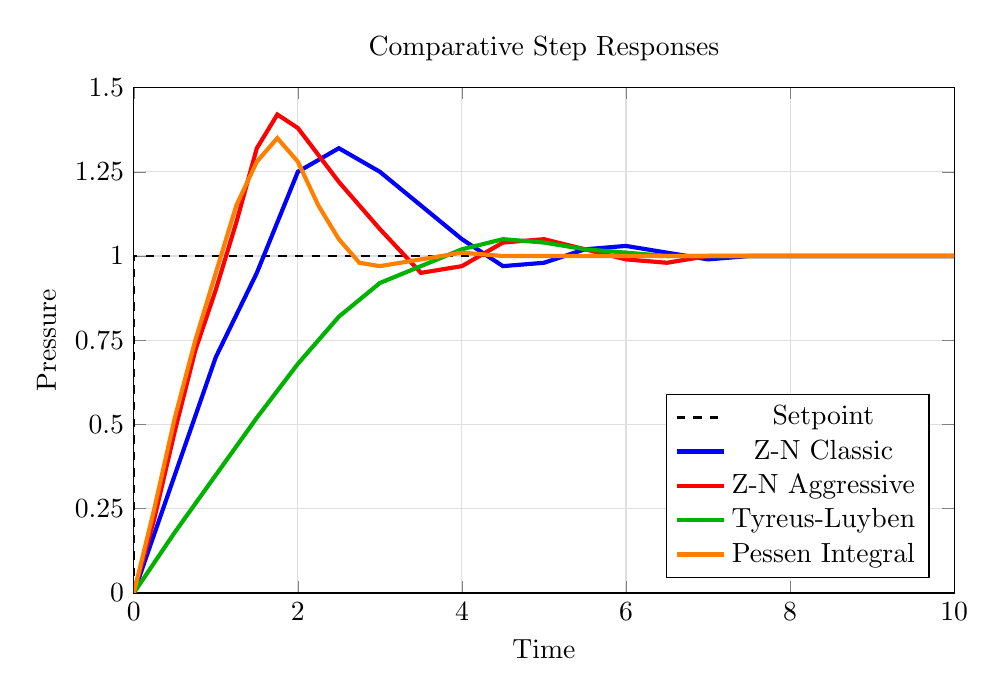
\begin{tikzpicture}
\begin{axis}[
    width=12cm,
    height=8cm,
    xlabel={Time},
    ylabel={Pressure},
    xmin=0, xmax=10,
    ymin=0, ymax=1.5,
    xtick={0,2,4,6,8,10},
    ytick={0,0.25,0.5,0.75,1.0,1.25,1.5},
    legend pos=south east,
    grid=both,
    minor grid style={gray!25},
    major grid style={gray!25},
    title={Comparative Step Responses},
    ]
    
    % Setpoint
    \addplot[black, dashed, line width=1pt] coordinates {(0,0) (0,1) (10,1)};
    
    % Ziegler-Nichols Classic - Moderate overshoot, moderate settling
    \addplot[blue, line width=1.5pt] coordinates {
        (0,0) (0.5,0.35) (1,0.7) (1.5,0.95) (2,1.25) (2.5,1.32) (3,1.25) 
        (3.5,1.15) (4,1.05) (4.5,0.97) (5,0.98) (5.5,1.02) (6,1.03) 
        (6.5,1.01) (7,0.99) (7.5,1.0) (8,1.0) (9,1.0) (10,1.0)
    };
    
    % Ziegler-Nichols Aggressive - Higher overshoot, faster rise
    \addplot[red, line width=1.5pt] coordinates {
        (0,0) (0.25,0.22) (0.5,0.48) (0.75,0.72) (1,0.9) (1.25,1.1) 
        (1.5,1.32) (1.75,1.42) (2,1.38) (2.5,1.22) (3,1.08) (3.5,0.95) 
        (4,0.97) (4.5,1.04) (5,1.05) (5.5,1.02) (6,0.99) (6.5,0.98) 
        (7,1.0) (8,1.0) (9,1.0) (10,1.0)
    };
    
    % Tyreus-Luyben - Less overshoot, slower rise and settling
    \addplot[green!70!black, line width=1.5pt] coordinates {
        (0,0) (0.5,0.18) (1,0.35) (1.5,0.52) (2,0.68) (2.5,0.82) (3,0.92) 
        (3.5,0.97) (4,1.02) (4.5,1.05) (5,1.04) (5.5,1.02) (6,1.01) 
        (6.5,1.0) (7,1.0) (8,1.0) (9,1.0) (10,1.0)
    };
    
    % Pessen Integral - Fast rise, moderate overshoot, quick settling
    \addplot[orange, line width=1.5pt] coordinates {
        (0,0) (0.25,0.25) (0.5,0.52) (0.75,0.75) (1,0.95) (1.25,1.15) 
        (1.5,1.28) (1.75,1.35) (2,1.28) (2.25,1.15) (2.5,1.05) (2.75,0.98) 
        (3,0.97) (3.5,0.99) (4,1.01) (4.5,1.0) (5,1.0) (6,1.0) (7,1.0) 
        (8,1.0) (9,1.0) (10,1.0)
    };

    \legend{Setpoint, Z-N Classic, Z-N Aggressive, Tyreus-Luyben, Pessen Integral}
\end{axis}
\end{tikzpicture}
\caption{Typical step responses for different tuning rules applied to the pressure control system. The plot shows how each rule affects rise time, overshoot, and settling characteristics.}
\label{fig:step_responses}
\end{figure}

The plot illustrates several important characteristics:

\begin{itemize}
    \item \textbf{Z-N Classic (blue)}: Shows a moderate rise time with significant overshoot (approximately 32\%) and some oscillation before settling.
    
    \item \textbf{Z-N Aggressive (red)}: Demonstrates the fastest rise time with the highest overshoot (approximately 42\%) but can take longer to fully settle due to more pronounced oscillations.
    
    \item \textbf{Tyreus-Luyben (green)}: Exhibits the slowest rise time but with minimal overshoot (approximately 5\%), making it ideal for applications where overshoot must be minimized.
    
    \item \textbf{Pessen Integral (orange)}: Provides a fast rise time with moderate overshoot (approximately 35\%) but settles more quickly than the Ziegler-Nichols methods, making it well-suited for setpoint tracking applications.
\end{itemize}

The aggressiveness factor in the Z-N Aggressive method can shift its response curve between the Classic and Aggressive profiles shown here, providing flexible tuning options.

\subsection{Practical Recommendations}

\begin{enumerate}
    \item Start with the default (Ziegler-Nichols Aggressive, aggressiveness=2.0)
    \item If the response is too sluggish:
    \begin{itemize}
        \item First try increasing aggressiveness: \texttt{TUNE AGGR 1.5} or \texttt{TUNE AGGR 2.0}
        \item If still insufficient, try Pessen Integral rule: \texttt{TUNE RULE 3}
    \end{itemize}
    \item If overshoot is problematic:
    \begin{itemize}
        \item First try reducing aggressiveness: \texttt{TUNE AGGR 0.8}
        \item If still insufficient, switch to Tyreus-Luyben: \texttt{TUNE RULE 2}
    \end{itemize}
    \item Enable anti-windup (\texttt{AW ON}) for all tuning methods to improve recovery from saturation
    \item For valves with significant stiction, enable hysteresis compensation (\texttt{HYST ON})
    \item After auto-tuning, fine-tune individual parameters if necessary:
    \begin{itemize}
        \item To reduce overshoot: reduce Kp or increase Kd
        \item To eliminate steady-state error: increase Ki
        \item To reduce oscillation: increase Kd or reduce Kp
    \end{itemize}
\end{enumerate}

\subsection{Limitations}

The auto-tuning method has several limitations to be aware of:

\begin{itemize}
    \item Works best for linear or approximately linear systems
    \item May not produce optimal results for highly non-linear systems
    \item Performance can be affected by noise (mitigated with AUTOTUNE\_NOISE\_BAND)
    \item Requires a stable starting point for best results
    \item External disturbances during tuning can affect accuracy
\end{itemize}

\section{Conclusion}

The VentCon2 system implements a sophisticated PID control system with advanced features like anti-windup and hysteresis compensation. The automated tuning procedure based on the relay method provides an accessible way to optimize the control parameters for specific applications without requiring in-depth knowledge of control theory\cite{astrom1995pid}.

The multiple tuning rules offer flexibility to balance between response speed, overshoot, and disturbance rejection based on the specific requirements of the application\cite{odwyer2009handbook}\cite{controlguru}\cite{controlnotes}\cite{oreilly:pidtuning}.

\nocite{*}  % Include all references, even if not explicitly cited

\section{References}

\begin{thebibliography}{99}

\bibitem{astrom1984automatic}
Åström, K.J. and Hägglund, T. (1984).
\newblock Automatic tuning of simple regulators with specifications on phase and amplitude margins.
\newblock \emph{Automatica}, 20(5):645--651.

\bibitem{ziegler1942optimum}
Ziegler, J.G. and Nichols, N.B. (1942).
\newblock Optimum settings for automatic controllers.
\newblock \emph{Transactions of the ASME}, 64:759--768.

\bibitem{tyreus1992tuning}
Tyreus, B.D. and Luyben, W.L. (1992).
\newblock Tuning PI controllers for integrator/dead time processes.
\newblock \emph{Industrial \& Engineering Chemistry Research}, 31(11):2625--2628.

\bibitem{pessen1954new}
Pessen, D.W. (1954).
\newblock A new look at PID-controller tuning.
\newblock \emph{Journal of Basic Engineering}, 76:494--501.

\bibitem{astrom1995pid}
Åström, K.J. and Hägglund, T. (1995).
\newblock \emph{PID Controllers: Theory, Design, and Tuning}.
\newblock Instrument Society of America, Research Triangle Park, NC, 2nd edition.

\bibitem{odwyer2009handbook}
O'Dwyer, A. (2009).
\newblock \emph{Handbook of PI and PID controller tuning rules}.
\newblock Imperial College Press, London, 3rd edition.

\bibitem{wiki:pid}
Wikipedia (2023).
\newblock PID controller.
\newblock \url{https://en.wikipedia.org/wiki/PID_controller}
\newblock [Online; accessed November 2023]

\bibitem{wiki:pidtuning}
Wikipedia (2023).
\newblock PID controller tuning.
\newblock \url{https://en.wikipedia.org/wiki/PID_controller#Loop_tuning}
\newblock [Online; accessed November 2023]

\bibitem{controlguru}
Control Guru (2023).
\newblock PID control and auto-tuning resource site.
\newblock \url{https://controlguru.com/}
\newblock [Online; accessed November 2023]

\bibitem{controlnotes}
MathWorks (2023).
\newblock PID Tuning Algorithms.
\newblock \url{https://www.mathworks.com/help/control/ug/pid-tuning-algorithms.html}
\newblock [Online; accessed November 2023]

\bibitem{oreilly:pidtuning}
Control Engineering Practice (2023).
\newblock PID Control Tuning: Principles and Applications.
\newblock \url{https://blog.opticontrols.com/archives/344}
\newblock [Online resource; accessed November 2023]

\bibitem{ni:pidtuning}
National Instruments (2023).
\newblock PID theory explained.
\newblock \url{https://www.ni.com/en-us/innovations/white-papers/06/pid-theory-explained.html}
\newblock [Online; accessed November 2023]

\end{thebibliography}

\end{document}
